\section{Behaviors}


Our bot uses behaviors tree (using the library from \cite{libbehavior}). 
An example of the behavior tree used by the units acheiving \texttt{Kitting\footnote{Staying at a distance, using ranged attacks, and running whenever the enemy comes near}} is depicted in Figure \ref{behaAttackClos}.

\begin{figure}[h!t]
\centering
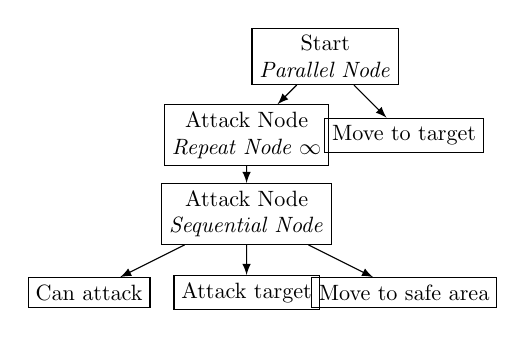
\begin{tikzpicture}[node distance = 1 cm]
    \tikzstyle{quadri}=[rectangle, align=center, scale=0.8, draw]
    \tikzstyle{link}=[->,thin,>=latex]
    \node[quadri] (start) at (0,3) {Start \\ \emph{Parallel Node}};
    \node[quadri] (repeatAttack) at (-1,2) {Attack Node \\ \emph{Repeat Node $\infty$}};
    \node[quadri] (leafMove) at (1,2) {Move to target};
    \node[quadri] (seqAttack) at (-1,1) {Attack Node \\ \emph{Sequential Node}};
    \node[quadri] (leafBool) at (-3,0) {Can attack};
    \node[quadri] (leafAttack) at (-1,0) {Attack target};
    \node[quadri] (leafFlee) at (1,0) {Move to safe area}; 
    \draw[link] (start)--(repeatAttack);
    \draw[link] (start)--(leafMove);
    \draw[link] (repeatAttack)--(seqAttack); 
    \draw[link] (seqAttack)--(leafBool);
    \draw[link] (seqAttack)--(leafAttack);
    \draw[link] (seqAttack)--(leafFlee);
\end{tikzpicture}
\caption{Behavior tree for kitting}
\label{behaAttackClos}
\end{figure}

